\chapter{Design and Implementation}
\label{chap:implementation}
Figure \ref{fig:three-tier-architecture} gives an overview of the three-tier architecture of the jSCAPE system, the relationships between each of the main components, and some of the tasks that they perform. The student view is implemented as a JavaFX applet embedded into the web browser. It communicates with a custom written Java application server using a custom built communication protocol. Finally, the application server also connects to a PostgreSQL database, to perform the standard read and write operations. \newline

\begin{figure}[H]
\centering
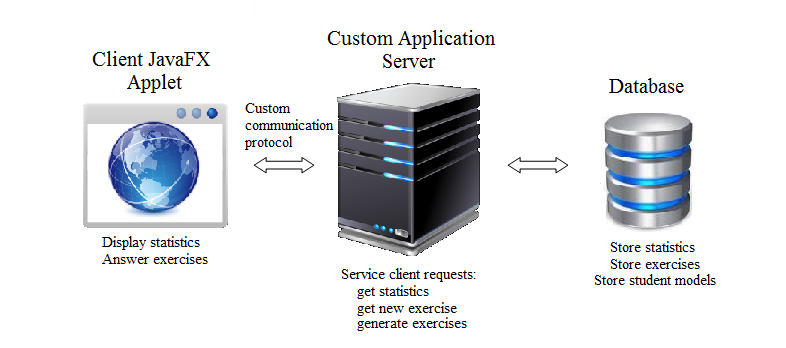
\includegraphics[width=\textwidth,height=\textheight,keepaspectratio]{three-tier-architecture}
\caption{Three tier architecture of the jSCAPE system.}
\label{fig:three-tier-architecture}
\end{figure}

The jSCAPE admin tool isn't really part of the core system's three tier architecture. The component was written later on to facilitate certain functions such as analyzing results and exercise bank management. To do so, it connects directly to the database to read or write information. The admin tool is shown in figure  \ref{fig:admin_tool_architecture}, along with its sub-components: the Results Analyzer, for displaying statistics in graphical form, and the Exercise Generator, for generating new exercises.

\begin{figure}[H]
\centering
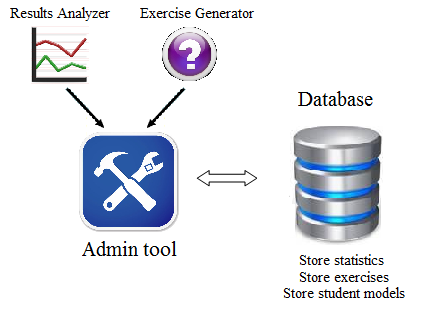
\includegraphics[scale=0.8]{admin_tool_architecture}
\caption{Architecture of the jSCAPE admin tool}
\label{fig:admin_tool_architecture}
\end{figure}

In the rest of this chapter we justify our design choices and discuss the implementation of the various components and features of the jSCAPE system.

\section{Technology choices}
Most software in the area of computer based education is web-based, as demonstrated by the review of related work in chapter \ref{chap:related-work}. We decided to follow this trend, as it makes deployment easier, and because students are usually quite familiar with web browsers. Therefore, the three-tier architecture of web client, server and database was the natural model of choice for creating such a system. There are multiple technologies which can be used to develop the client side. Some of these are HTML5, CSS, Javascript, Flash, and Java applets.\newline

We decided to take the approach of Java applets because we have had a lot of experience with developing large scale programs in this language. In addition, in our opinion, Java applets are better for creating rich web applications which resemble desktop applications. Websites require the user to continuously click links, and load web pages to access a feature, and we think that this model isn't suitable for developing jSCAPE. Finally, implementing jSCAPE as an applet allows it to run in Java web start mode or as a stand alone desktop application, thanks to the Java deployment framework. \newline

However, regular Java applets use the Swing library for GUIs, and as a result, the interface doesn't end up being user-friendly or visually appealing. This is certainly a problem, because although the application can present powerful and useful features, students will only use it if the interface is intuitive and aesthetically pleasing\cite{Interface-study}. \newline

This realisation led us to researching libraries which could improve the interfaces of Java applets, and discovering JavaFX. JavaFX is intended as a replacement for the Swing GUI library, and is designed to provide a lightweight, hardware-accelerated Java UI platform for creating rich internet applications\cite{JavaFX}. The JavaFX library includes a powerful and visually appealing statistics package, with support for pie charts, bar charts, line charts, scatter charts, tables, etc... which was more than enough to implement the statistics tracking and displaying component of jSCAPE. In addition, this would allow us to easily add more displayable statistics in the future (section \ref{sec:future-work}), if required. \newline

JavaFX also provides the functionality of embedding a \textsf{WebView}, a browser component which supports HTML5, CSS and Javascript, into the applet. We found that this could be an interesting feature to use for developing exercises with variety and interactivity, For instance, this component is used in the Binary Tree exercises to display the binary trees (section 5.??). \newline

Every web application needs some sort of server to handle web client requests. We looked at Java Server Pages (JSP) and Java Servlets, but the setup and organization required to make them work seemed to be too much work for the very little advantages they offered. Instead we opted to write our own Java server because this would offer more control for handling requests and more flexibility for extensions in the future. In addition, the time and amount of code required to write a functional server was very minimal. Indeed, the basic components of our custom built server fit into approximately 300 lines of code. \newline

A database is needed for permanent storage of the system's state, student models, exercises, etc... Thus, to do this, we use a PostgreSQL database and connect to it using the associated Java Database Connectivity (JDBC) driver. \newline

Throughout this chapter, we will give more detail about which tables are maintained by the system, and how they are used. In addition, we will introduce some other technologies and libraries used in this project later on, when we look at the exercise generation and display processes.
\section{Design}
This section describes the design of the jSCAPE system.

\subsection{Client}
\begin{figure}[H]
\centering
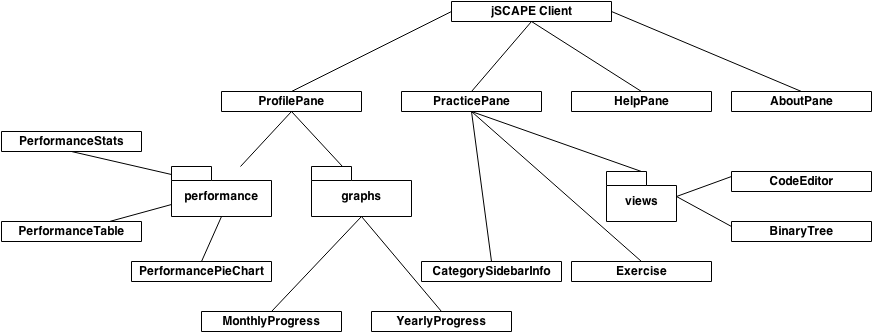
\includegraphics[width=\textwidth,height=\textheight,keepaspectratio]{class_diagram_client}
\caption{Class diagram of the jSCAPE client.}
\label{fig:class_diagram_client}
\end{figure}

Figure \ref{fig:class_diagram_client} shows the class diagram of the jSCAPE client, which is what is embedded into the web browser, and displayed to students. We briefly describe the classes:
\begin{itemize}
\item \textsf{ProfilePane}: The Profile tab of the application.
      \begin{itemize}
      \item[-] \textsf{performance} package:
               \begin{itemize}
               \item[-] \textsf{PerformanceStats}: Stores performance statistics, i.e. exercise category, correct answers, wrong answers.
               \item[-] \textsf{PerformanceTable}: Table wrapper to display \textsf{PerformanceStats} objects.
               \item[-] \textsf{PerformancePieChart}: PieChart wrapper to display \textsf{PerformanceStats} objects.
               \end{itemize}
      \item[-] \textsf{graphs} package:
               \begin{itemize}
               \item[-] \textsf{MonthlyProgress}: StackedBarChart wrapper to display monthly progress statistics.
               \item[-] \textsf{YearlyProgress}: StackedBarChart wrapper to display yearly progress statistics.
               \end{itemize}
      \end{itemize}
\item \textsf{PracticePane}: The Practice tab of the application.
       \begin{itemize}
       \item[-] \textsf{Exercise}: Stores an exercise and information such as exercise ID, description, choices, solution, display values.
       \item[-] \textsf{CategorySidebarInfo}: Stores information to create the sidebar of an exercise window.
       \item[-] \textsf{views} package contains the classes to render exercises in the left part of the Practice tab:
                \begin{itemize}
                \item[-] \textsf{BinaryTree}: Component capable of drawing binary trees.
                \item[-] \textsf{CodeEditor}: Component capable of displaying programming code in a code editor.
                \end{itemize}
       \end{itemize}

\item \textsf{HelpPane}: The Help tab of the application, displays the manual.

\item \textsf{AboutPane}: The About tab of the application, displays information about what the application does.
\end{itemize}

The jSCAPE client accounts for approximately 2500 lines of code.

\subsection{Server}
\begin{figure}[H]
\centering
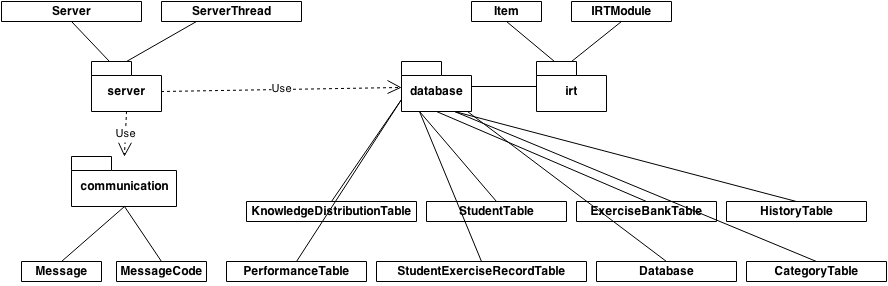
\includegraphics[width=\textwidth,height=\textheight,keepaspectratio]{class_diagram_server}
\caption{Class diagram of the jSCAPE server.}
\label{fig:class_diagram_server}
\end{figure}

Figure \ref{fig:class_diagram_server} shows the class diagram of the jSCAPE server, and the database classes the server uses to satisfy client requests. We briefly describe the classes:
\begin{itemize}
\item \textsf{server} package:
      \begin{itemize}
      \item[-] \textsf{Server}: The server, creates \textsf{ServerThread}s to handle client connections.
      \item[-] \textsf{ServerThread}: Receives requests from the client(s), performs work and replies to the client(s).
      \end{itemize}
\item \textsf{communication} package:
      \begin{itemize}
      \item[-] \textsf{Message}: A data structure to hold information. This is the unit which ``travels" between the client and server, and vice-versa.
      \item[-] \textsf{MessageCode}: Enum to identify structure and format of a \textsf{Message}.
      \end{itemize}     
\item \textsf{database} package:
      \begin{itemize}
      \item[-] \textsf{Database}: Manages the connection info and hands out connections to the components that wish to access the physical database.
      \item[-] \textsf{StudentTable}: Stores profile information of students, login names, passwords, etc...
      \item[-] \textsf{CategoryTable}: Stores the exercise categories, their description and associated lecture notes or helpful website links.
      \item[-] \textsf{PerformanceTable}: Stores performance statistics, such as correct answers and wrong answers, of students for the different exercise categories.
      \item[-] \textsf{HistoryTable}: Stores performance statistics of students for each day they used the system.
      \item[-] \textsf{ExerciseBankTable}: Stores the exercises, some exercise metrics and difficulty parameters.
      \item[-] \textsf{StudentExerciseRecordTable}: Stores which exercises students have answered and whether they got it correct or incorrect.
      \item[-] \textsf{KnowledgeDistributionTable}: Stores the knowledge distribution of the student per exercise category, in the case that Item Response Theory is used.
      \end{itemize}
\item \textsf{irt} package: This package is a Java implementation of Item Response Theory.
      \begin{itemize}
      \item[-] \textsf{Item}: An IRT item, which stores an exercise ID and item parameters.
      \item[-] \textsf{IRTModule}: Implements IRT concepts such as the item response function, the item information function, ability estimation, etc...
      \end{itemize}
\end{itemize}

\subsection{Exercises and exercise generators}
\begin{figure}[H]
\centering
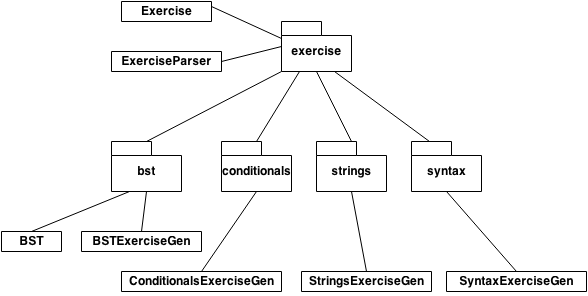
\includegraphics[width=\textwidth,height=\textheight,keepaspectratio]{class_diagram_exercises}
\caption{Class diagram of the currently implemented exercise generators.}
\label{fig:class_diagram_exercises}
\end{figure}

Figure \ref{fig:class_diagram_exercises} shows the class diagram for exercises and the implemented exercise generators, at the time of writing this report. We briefly describe the classes:
\begin{itemize}
\item \textsf{Exercise}: Stores an exercise and information such as exercise ID, description, choices, solution, display values.
\item \textsf{ExerciseParser}: Special XML parser to decode the exercise format and return an \textsf{Exercise}.
\item \textsf{bst} package:
      \begin{itemize}
      \item[-] \textsf{BST}: Java implementation of binary trees with standard functions such as insert, traversal, height, etc...
      \item[-] \textsf{BSTExerciseGen}: Generates an exercise for the Binary Tree exercise category.
      \end{itemize}
\item \textsf{conditionals} package:
      \begin{itemize}
      \item[-] \textsf{ConditionalsExerciseGen}: Generates an exercise for the Conditionals exercise category.
      \end{itemize}
\item \textsf{strings} package:
      \begin{itemize}
      \item[-] \textsf{StringsExerciseGen}: Generates an exercise for the Strings exercise category.
      \end{itemize}
\item \textsf{syntax} package:
      \begin{itemize}
      \item[-] \textsf{SyntaxExerciseGen}: Generates an exercise for the Syntax exercise category.
      \end{itemize}                 
\end{itemize}

\subsection{Admin tool}
We won't go into the details of the admin tool design. Essentially it reuses classes from other components and adds a few modifications.\newline

This component accounts for approximately 2000 lines of code, although most of those lines are copied from other components.

\section{Server and client-server communication}
The server is responsible for servicing all client requests, for instance, requesting performance statistics or requesting a new exercise. It is custom built, multithreaded and written in pure Java, using Sockets and Object input/output streams. The basic server class and the mechanism to communicate with clients accounts for approximately 300 lines of code. \newline

\lstinputlisting[language=Java, caption={Serializable message object used for client-server communication.}, label={lst:message.java}]{\listings/message.java}
The code in \ref{lst:message.java} shows the basic unit that travels between the client and the server, and vice-versa. A message consists of a message code, used to determine its structure, and a payload of request parameters, in the form of an \textsf{ArrayList$<$String$>$}.\newline

The existing message request codes are shown in \ref{lst:message_codes.java}. The server uses these to determine what the client has requested, how the request message is formatted and which actions to perform to service the request. \newpage

\lstinputlisting[language=Java, caption={Message request codes.}, label={lst:message_codes.java}]{\listings/message_codes.java}

The code snippet in \ref{lst:example_service.java} gives an example of how the client can construct a request. In this particular example the client is requesting the statistical data about the student's performance. On line 1, a \textsf{Service} is created. A \textsf{Service} is a task that can be performed over and over again by calling the \textsf{restart()} method, like on line 12. Lines 2 to 10 determine what the service should do when it is started. Lines 4 and 5 add the student's login name as a request parameter. On lines 6 and 7, the message is constructed with the appropriate message code, and the request parameters. On line 9, the message is sent to the server, and the reply from the server is stored in the \textsf{Service}, for the client to use later on.\newline

\lstinputlisting[language=Java, caption={An example client request.}, label={lst:example_service.java}]{\listings/example_service.java}

In addition to communicating with the client, the server also communicates with the PostgreSQL database. This is to retrieve the data requested by the client, and to update the state of the system as the student answers exercises, for instance. Therefore, a database module was created with methods to perform the necessary functions. \newline

\lstinputlisting[language=Java, caption={An example database retrieval method.}, label={lst:example_database_method.java}]{\listings/example_database_method.java}

In listing \ref{lst:example_database_method.java} we give an example of a database retrieval method. Such methods form a large part of the database module. All methods which read from the database return a \textsf{ArrayList$<$String$>$}, so that this can be immediately put in the reply message from the server to the client. In this particular example, the method retrieves performance statistics for the student identified by \textsf{loginName}. Line 6 creates the data structure to hold the information which will be read from the database. Lines 8 to 18 create the query, and send it to the database to be executed. In lines 20 to 24, the result of the query is added to the data structure. Finally, on line 27, all this information is returned to the server, which can now encapsulate this in a reply message, and send that to the client.\newline

The database module also includes methods to update the information stored in the database. These methods simply execute an SQL \textsf{UPDATE} query, and return no status. \newline

This database module is also used by the jSCAPE admin tool to analyze results and manage the exercise bank. The module comprises of 8 classes, one main database class and one for each database table, and accounts for approximately 1500 lines of code.

%talk about Beanshell for ex gen
\section{Exercises}
The possibility to practice understanding of programming concepts through exercises can be considered jSCAPE's central feature. In this section we discuss some of the design considerations for exercises, how they are implemented in jSCAPE and how exercise generators can be written to automatically generate these exercises.

\subsection{Design choices}
The fact is that with jSCAPE's flexible exercise format, it is possible to handle multiple types of exercise. However, instead of trying to include a large number of exercises, we decide to focus on a limited amount of exercises and get things right.

Java programming exercises, focus on one language, to illustrate system, system is pretty much language independent.

Multiple choice questions for 3PL IRT model.

no exercises asking to write code because students usually have labs to do that, and these exercises are intended to practice understanding of fundamentals and to reinforce mental models of what programming language constructs actually do.

showing feedback immediately afterwards...piece of code+exercise for code semantics understanding.

We decided to have at least two different types of exercises to show the capabilities of the system in handling multiple exercise types.

\subsection{jSCAPE exercise format}
To represent an exercise entity, jSCAPE uses a simple XML tagged document. This is shown in listing \ref{lst:exercise_format}.\newline

\lstinputlisting[language={xml}, tabsize=4, caption={Exercise format.},label={lst:exercise_format}]{\listings/exercise_format.xml}

To understand the format, recall how exercises are displayed to students in the Practice tab (section \ref{subsec:pratising-programming}). Exercise data is shown in the left window, and the exercise description and choices are shown in the right window.
We now explain the significance of these tags:
\begin{itemize}
\item The first \textsf{$<$display$>$} tag encloses information about the left window. The enclosed \textsf{$<$view$>$} tag corresponds to the component required to render the exercise data in the left window. Currently, two values are possible for this tag, \textsf{BinaryTree} and \textsf{CodeEditor}. The enclosed \textsf{$<$value$>$} tag holds the data that is passed to the rendering component to be rendered accordingly.
\item The second \textsf{$<$display$>$} tag encloses information about the right window. The enclosed \textsf{$<$view$>$} tag corresponds to the type of exercise, and currently only one value is possible, \textsf{Multiple Choice}. The enclosed \textsf{$<$value$>$} tag holds the exercise description, i.e. the question asked. The \textsf{$<$choice$>$} tags correspond to the possible choices given to the student, and finally, the \textsf{$<$solution$>$} tag contains the solution to the exercise.
\item The last \textsf{$<$display$>$} tag encloses a \textsf{$<$difficulty$>$} tag which gives the difficulty category of the exercise. Details about the difficulty category parameter will be given in the next section, on exercise generation.
\end{itemize}

Some examples of jSCAPE exercises are shown in appendix \ref{chap:example-jscape-exercises}.

\subsection{Exercise generation}
\label{exercise-generation}

\section{Implementing Computerized Adaptive Testing (CAT)}
We refer back to the background section where we outlined the components of a CAT. We also base this section on the work of SIETTE, for the reasons outlined in the related work section. We will use, bayesian estimation with knowledge distributions. 12 discrete knowledge levels, 0 to 11, as in SIETTE, no starting point, modified termination criterion, and three different item selection algorithms.

\subsection{Calibrated item pool}

\subsection{Starting point}
The starting point refers to the state of the system when no exercises have been administered to a student. In jSCAPE, no prior information about students is known, so the system's initial ability estimate for the student corresponds to the mean on the ability scale, i.e. $\theta = 5$. In addition, the initial knowledge distribution will be a uniform distribution with $P(\theta)=\frac{1}{11}$, where $P(\theta)$ is the probability that the student's knowledge level is equal to $\theta$. These initial assumptions are taken for every exercise category.

\subsection{Implementing exercise selection algorithms}

\subsubsection{Random selection}
Random selection

\subsubsection{Selecting based on the difficulty category}

\begin{figure}[H]
\centering
\begin{tikzpicture}[>=stealth',shorten >=1pt,auto,node distance=3cm]
  \node[initial,state] (A1)      {$A1$};
  \node[state]         (A2) [right of=A1]  {$A2$};
  \node[state]         (A3) [right of=A2] {$A3$};
  \node[state]         (B1) [below of=A3] {$B1$};
  \node[state]         (B2) [left of=B1] {$B2$};
  \node[state]         (B3) [left of=B2] {$B3$};
  \node[state]         (C1) [below of=B3] {$C1$};
  \node[state]         (C2) [right of=C1] {$C2$};
  \node[state]         (C3) [right of=C2] {$C3$};


  \path[->] (A1)  edge [loop above] node {wrong} (A1)
             edge [bend left] node {correct} (A2)
        (A2) edge [bend left]  node {wrong} (A1)
             edge [bend left] node {correct} (A3)
        (A3) edge [bend left]  node {wrong} (A2)
             edge [bend left] node {correct} (B1)
        (B1) edge [bend left]  node {wrong} (A3)
             edge [bend left] node {correct} (B2)
        (B2) edge [bend left]  node {wrong} (B1)
             edge [bend left] node {correct} (B3)
        (B3) edge [bend left] node {wrong} (B2)
             edge [bend left] node {correct} (C1)
        (C1) edge [bend left] node {wrong} (B3)
             edge [bend left] node {correct} (C2)
        (C2) edge [bend left] node {wrong} (C1)
             edge [bend left] node {correct} (C3)
        (C3) edge [loop above] node {correct} (C3)
             edge [bend left] node {wrong} (C2);             
\end{tikzpicture}
\caption{State machine of adaptive difficulty categories.}
\label{state-machine}
\end{figure}

Figure \ref{state-machine} shows the state machine implemented by this exercise selection algorithm.

\subsubsection{Selecting using Item Response Theory}

\lstinputlisting[language=Java, caption={Item information algorithm.}]{\listings/item_information.java}

\lstinputlisting[language=Java, caption={Item response function algorithm.}]{\listings/item_response_function.java}

\subsection{Scoring algorithm}

\subsection{Termination criterion}
When discussing CATs, we mentioned the need for a termination criterion. However, for jSCAPE we wanted no limit to be imposed on the number of exercises a student could answer. As long as exercises are available in the exercise bank, and as long as a student wants to practice, then he will be able to do so.\newline

The only termination criterion per say, is when a student exits an exercise category to practice exercises of another category. This means that when a student goes back to that previous exercise category, his knowledge distribution will continue to evolve from where it left off. A teacher could, for instance, reset the knowledge distribution every week or month to get more accurate and recent estimates of a student's knowledge.

\section{Collecting statistical data}
One of the main features of jSCAPE is tracking student progress through statistical data. In this section we briefly look at what statistical data is collected and how it is organized in the database.

\begin{figure}[H]
\centering
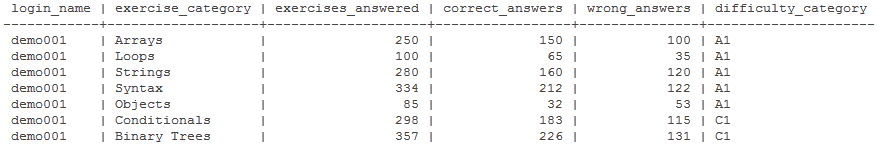
\includegraphics[width=\textwidth,height=\textheight,keepaspectratio]{performance_database_table}
\caption{Performance database table.}
\label{fig:performance_database_table}
\end{figure}

Figure \ref{fig:performance_database_table} shows that, for every student, the system records the number of exercises answered, the number of correct answers and the number of wrong answers for each exercise category defined by the teacher. In addition, the system keeps track of what difficulty category the student has reached for every exercise category. This is the information that gets displayed in the pie charts and performance table.

\begin{figure}[H]
\centering
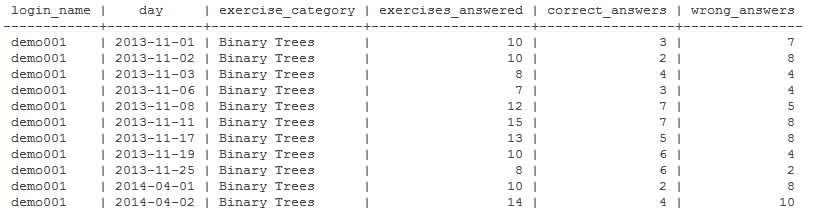
\includegraphics[width=\textwidth,height=\textheight,keepaspectratio]{history_database_table}
\caption{History database table.}
\label{fig:history_database_table}
\end{figure}

Figure \ref{fig:history_database_table} shows that the system records, for every student, the days where exercises were answered, the number of exercises answered answered on that day, the number of correct answers and the number of wrong answers, for every exercise category. This data is used to plot the stacked bar charts of monthly and yearly progress.

\begin{figure}[H]
\centering
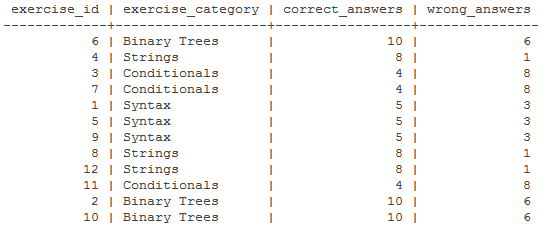
\includegraphics[width=\textwidth,height=\textheight,keepaspectratio]{exercisebank_database_table}
\caption{Exercise bank database table.}
\label{fig:exercisebank_database_table}
\end{figure}

Figure \ref{fig:exercisebank_database_table} shows that the system records the number of correct answers and wrong answers for each exercise. This is a useful feature for teachers to identify trends in which type of exercises students are having trouble with and which type of exercises students are having little trouble answering correctly.

\section{Summary}

\newpage

Talk about design choices such as only multiple choices, no exercises asking to write code, writing custom server, etc...\newline

java programming exercises, binary trees and code exercises to show the capabilities of the system, that it can handle multiple types of exercises.\newline

showing feedback immediately after the exercise....cite source, shown to be most effective way of learning\newline

piece of code + exercise involving the behaviour of the code have been found efficient (lister 2001) as far as student's assessment on their ability to read and understand the code's semantics. (NOT MY OWN WORDS) Lister, R. (2001). Objectives and objective assessment in CS1. ACM SIGCSE Bulletin, Vol. 33, No. 1, pp. 292-296. \newline

CAT development, we refer back to the five components of a CAT...what item selection algorithm we use, what scoring procedure, no termination criterion, entry point is average knowledge distribution initially and attempts at a calibrated item pool, currently with teacher providing the parameters since obtaining a high quality calibrated item pool isn't something I can do.
